\begin{frame}
	\frametitle{Unprotected Loss of Heat Sink}
		\textbf{Problem Description}
			\begin{itemize}
				\item \gls{ULOHS} accidents generally occur due to various causes
				of failure in the heat exchanger or secondary coolant loop
				\item In this work, \gls{ULOHS} is simulated by an exponential
				decrease in the heat loss rate from the heat exchanger with a
				time constant of 5 s
				\item Expect to observe a rise in temperature, accompanied by a
				decrease in neutron flux and heat generation
			\end{itemize}
\end{frame}

\begin{frame}
	\frametitle{Unprotected Loss of Heat Sink}
		\textbf{Results}
		\begin{columns}
			\column{5cm}
			\begin{figure}
				\centering
				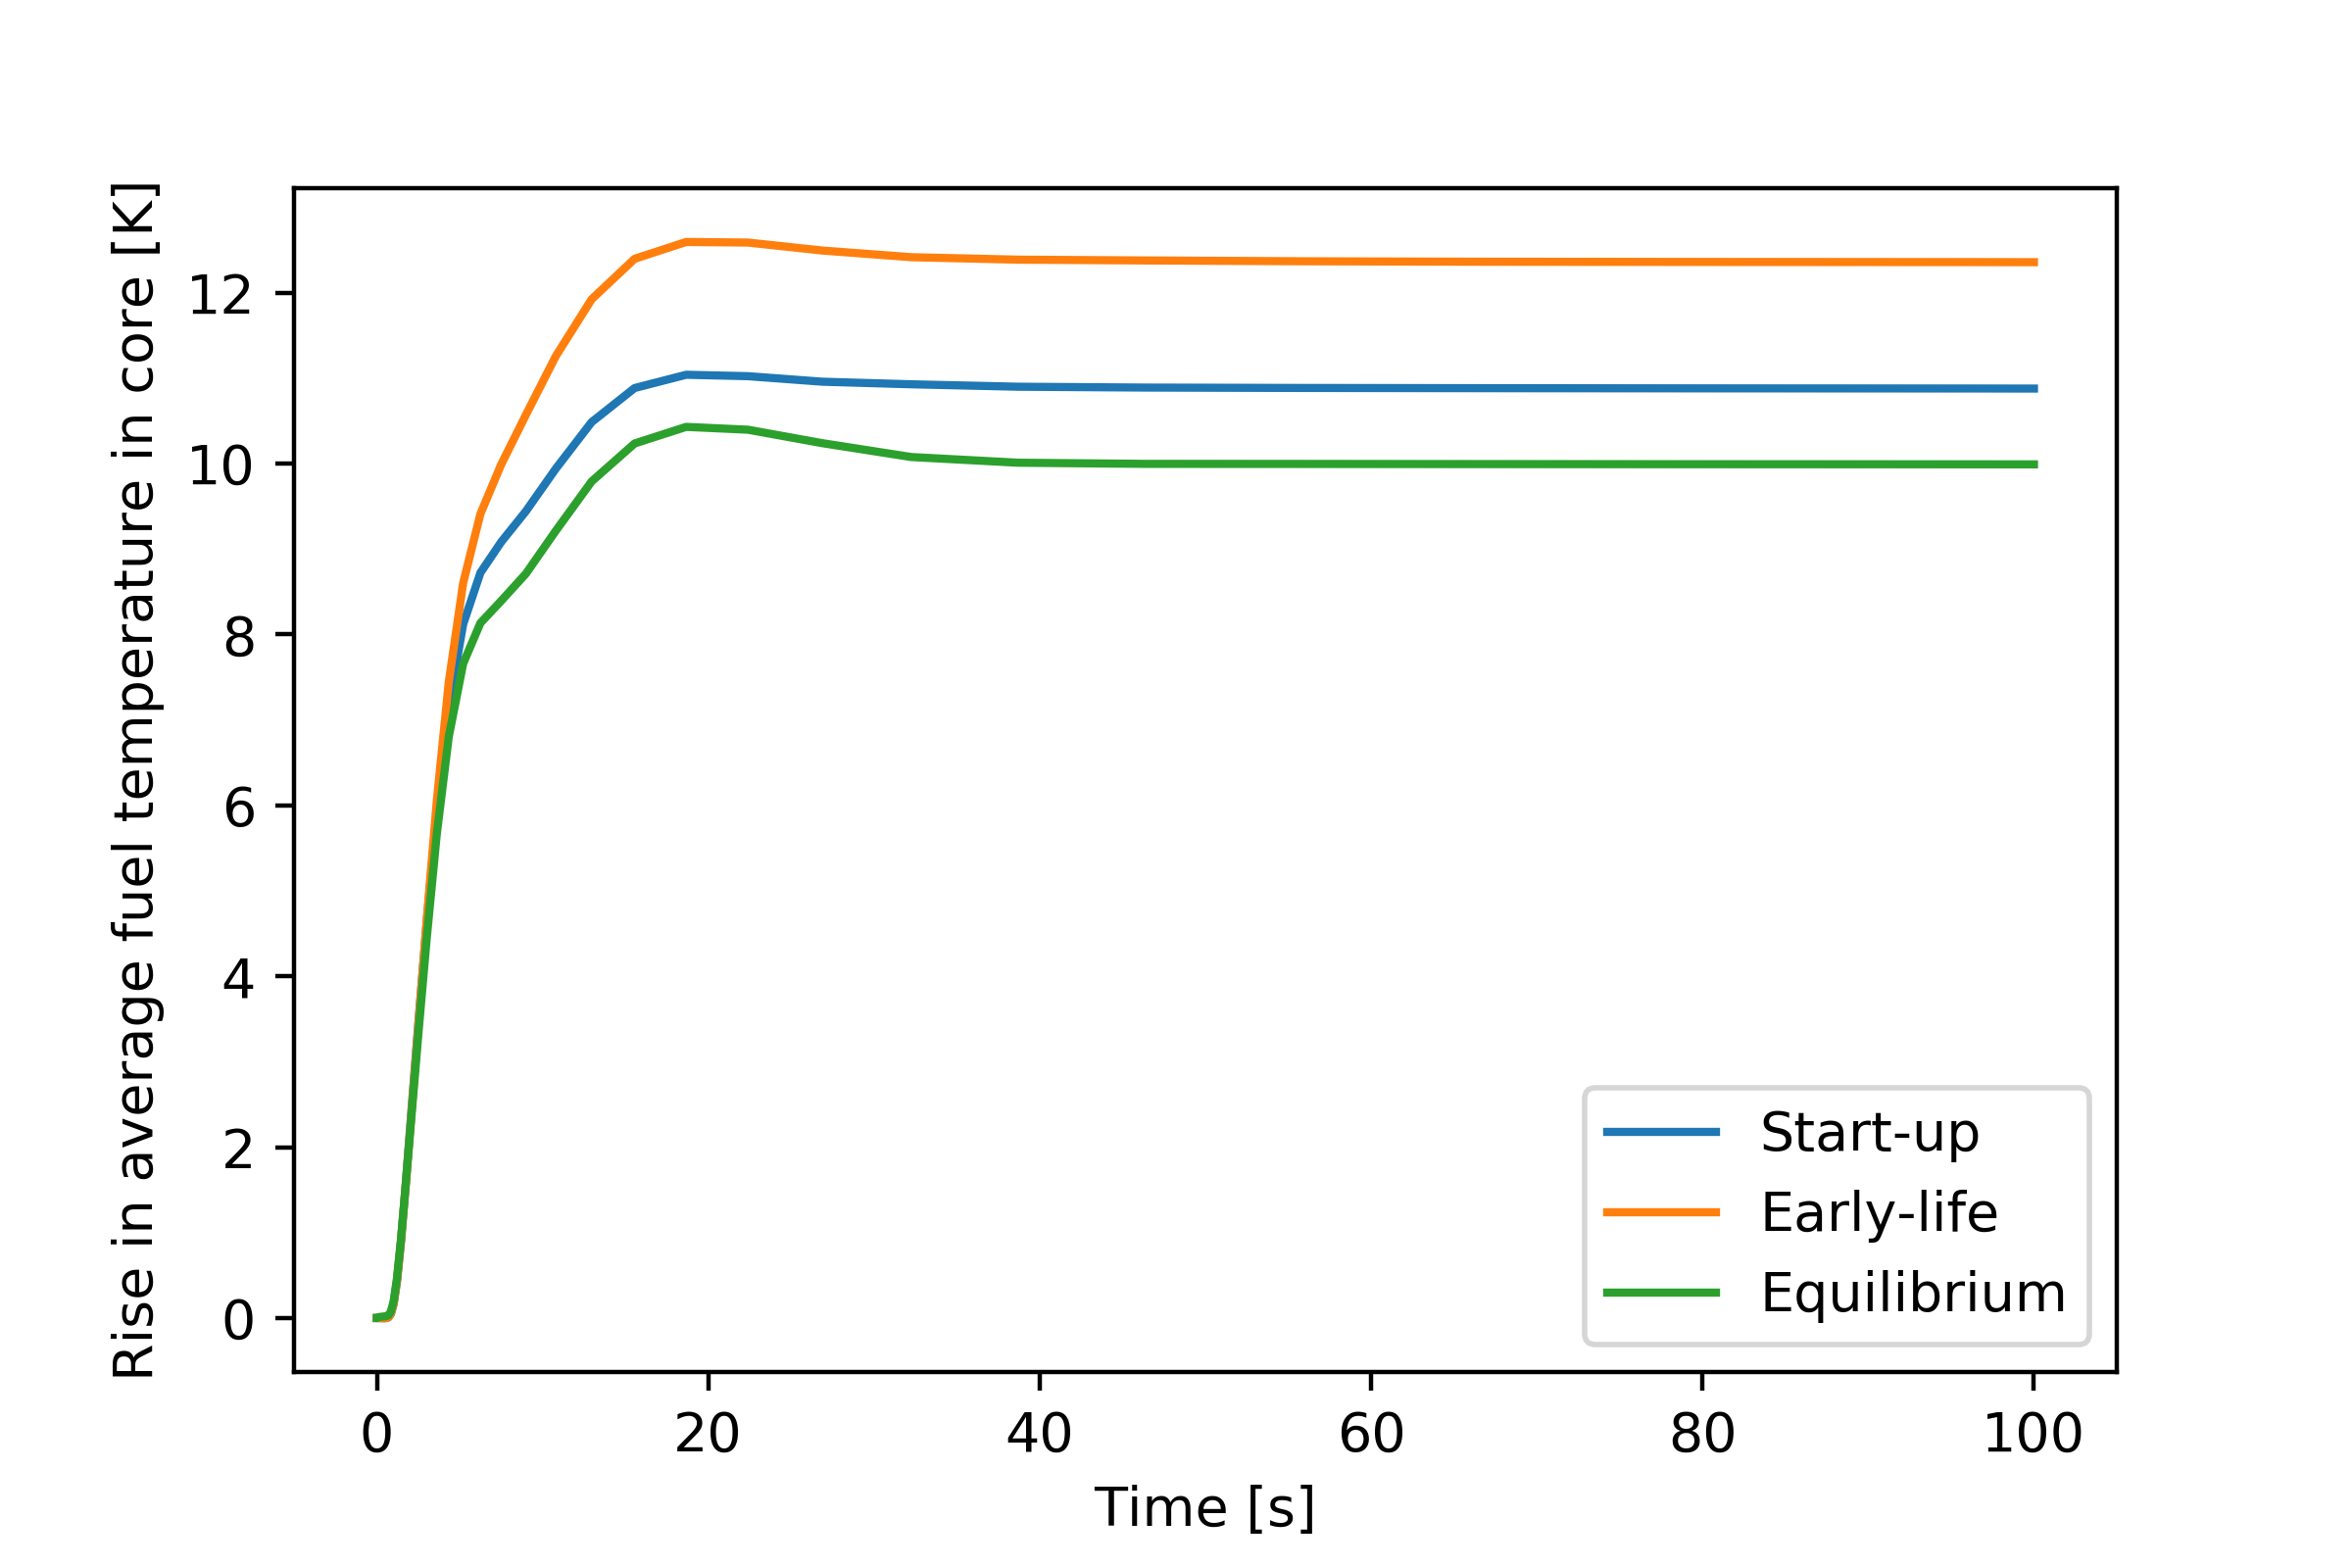
\includegraphics[width=\textwidth]{../paper/figures/loscatemp}
				\caption{Rise in average core temperature during \gls{ULOHS}}
			\end{figure}
			\column{5cm}
			\begin{figure}
				\centering
				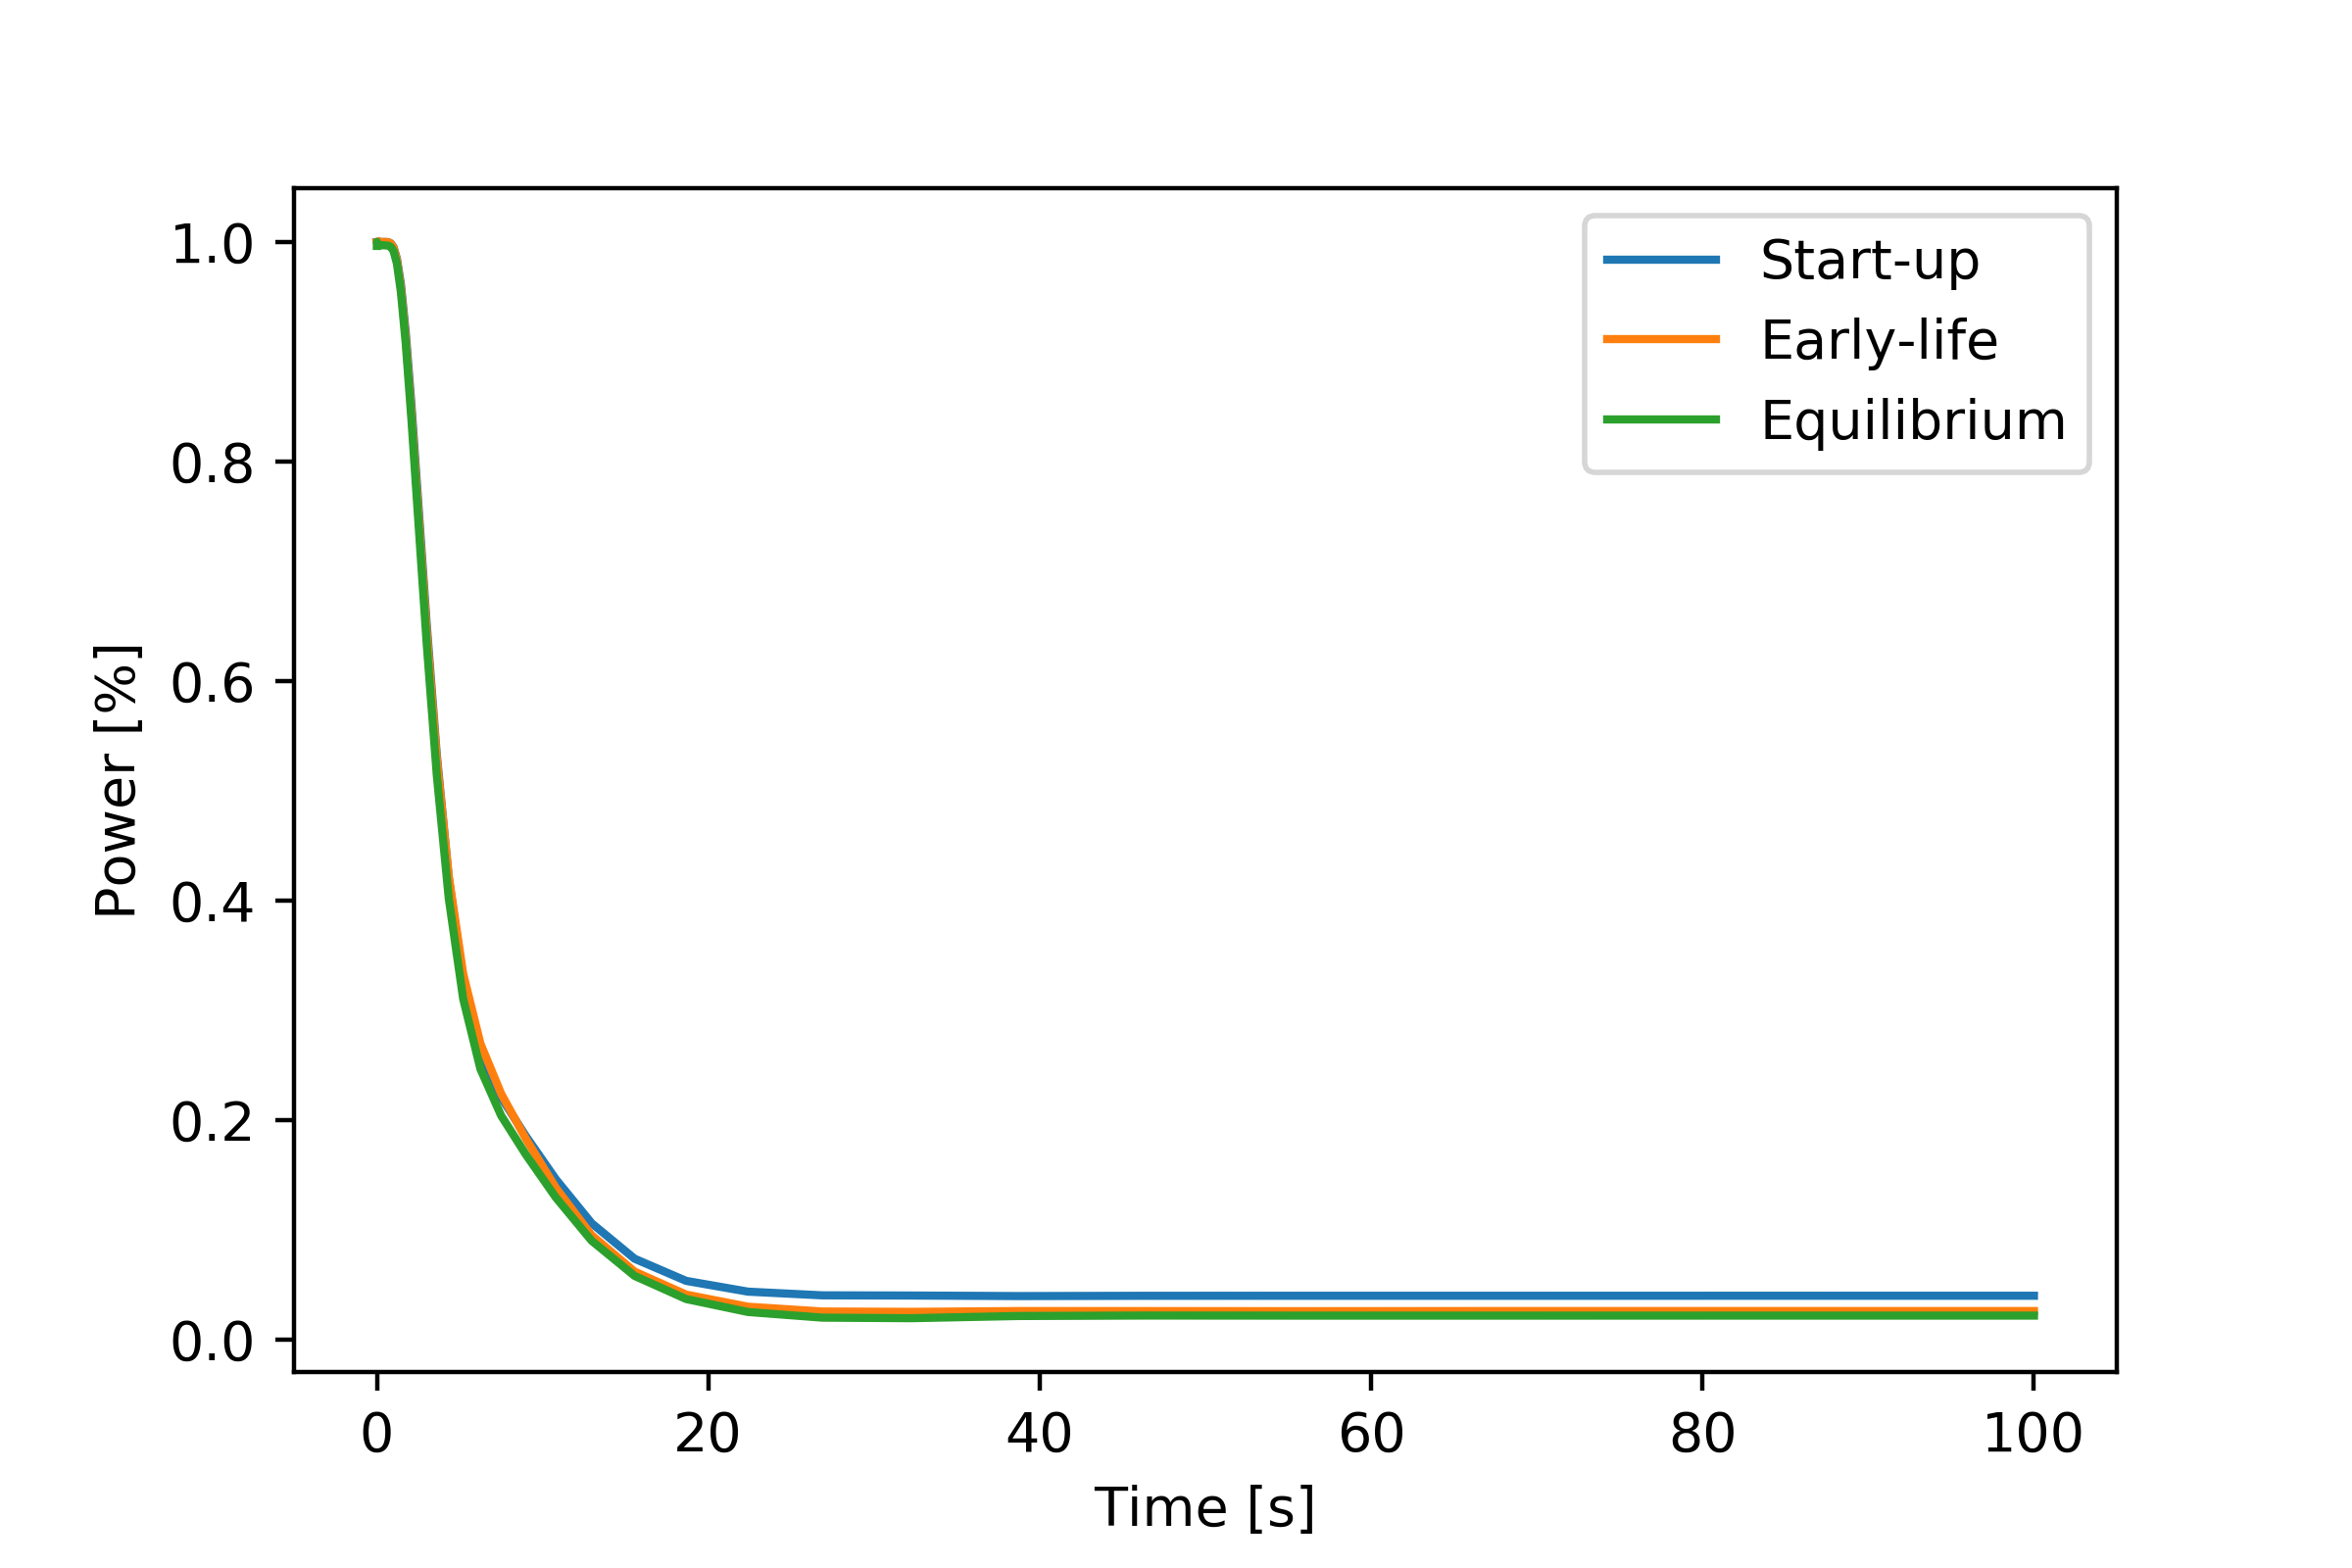
\includegraphics[width=\textwidth]{../paper/figures/loscaheat}
				\caption{Power generation during \gls{ULOHS}}
			\end{figure}
		\end{columns}
		\begin{itemize}
			\item \gls{ULOHS} starts at t = 0
			\item Average fuel temperature in core stabilizes at 10 K higher than
			the initial temperature
			\item Lower than expected temperature increase as decay heat is not
			modeled
		\end{itemize}
\end{frame}
